\documentclass[12pt,letterpaper]{article}

\marginparsep 0pt
\textwidth 6in
\topmargin 0pt
\headsep .5in
\textheight 8.7in
\voffset = 0pt
\hoffset = 0pt
\marginparwidth = 0pt
\oddsidemargin = 0pt

\usepackage[utf8]{inputenc}
\usepackage[spanish]{babel}
\usepackage{graphicx}
\usepackage{graphics}
\usepackage[dvips]{epsfig}
\usepackage[dvips]{graphicx}
\usepackage{rotating}
\usepackage{multirow}
\usepackage{array}
\usepackage{longtable}
\usepackage[]{fontenc}
\usepackage[nottoc,notlot,notlof]{tocbibind}


\addto\captionsspanish{
\def\listtablename{\'Indice de tablas}
\def\tablename{Tabla}
}

\begin{document}
\begin{center}
\begin{figure}[ht]
\begin{center}

\includegraphics[width=4cm]{logoUV.png}
\end{center}
\end{figure}
\thispagestyle{empty}

UNIVERSIDAD DE VALPARA\'ISO \\
Facultad de Ingenie\'ia \\
Escuela de Ingenier\'ia Civil en Inform\'atica \\
Ingenier\'ia Civil Inform\'atica\\
\vspace{1cm}
\Large
\textbf{Herramienta para la recolecci\'on de indicadores de comportamiento en ni\~nos con autismo 
mediante tecnolog\'ia de interacci\'on natural}\\ 
\large 
Propuesta de Trabajo de T\'itulo \\
Diozel Bernardo Zepeda Bruna \\
\normalsize
\emph{diozel.zepedab@alumnos.uv.cl} \\
\today \\
\vspace{1cm}
Profesor Gu\'ia:
REN\'E NO\"EL L\'OPEZ
\end{center}



\begin{abstract}


El diagnostico de los trastornos del espectro autista (TEA), conlleva un proceso largo 
y un trabajo constante de un grupo multidisciplinario de profesionales, que a partir de 
su experiencia y de estudios clasifican y caracterizan el comportamiento de cierto individuo. 
El uso de la tecnolog\'ia es algo nuevo, la utilizaci\'on de esta apoya la eficacia de la 
formaci\'on basada en computadoras, para la ense\~nanza de una serie de habilidades en los 
ni\~nos con TEA \cite{REF1}, pero a partir del uso de la tecnolog\'ia, no se obtiene informaci\'on 
respecto a la interacci\'on del ni\~no con el dispositivo, informaci\'on como por ejemplo, 
tiempo en que el ni\~no termina la actividad planteada o reacci\'on ante determinado objeto. 
Estos podr\'ian ser parte de un conjunto mayor de indicadores que podr\'ian ser de inter\'es 
para los especialistas. El presente trabajo propone la creaci\'on de una plataforma para 
capturar, almacenar y en un an\'alisis futuro, entregar informaci\'on valiosa para los 
especialistas, utilizando estos indicadores capturados y almacenados.


\end{abstract}



\newpage

\tableofcontents
\newpage

\listoftables
\listoffigures
\newpage



\section{Introducci\'on}
\label{intr}


En la siguiente propuesta de trabajo de t\'itulo (TT), el problema que se aborda 
tiene relaci\'on con el Trastorno de espectro Autista o TEA, este trastorno se 
define como una desarmon\'ia generalizada en el desarrollo de las funciones 
cognitivas superiores e independiente del potencial intelectual inicial. 
Estos ni\~nos presentan dificultades cualitativas en \'areas del lenguaje y 
la comunicaci\'on social y un rango de intereses restringido y repetitivo. 
El t\'ermino trastorno en el espectro autista (TEA) incluye trastorno autista 
(TA), S\'indrome de Asperger (SA) y trastornos perturbadores del desarrollo 
no especificados (TPDNE), seg\'un dsm-IV, CIE-10 \cite{REF2} \cite{REF6} \cite{REF7}, 
en la nueva publicaci\'on el DSM-V, el trastorno de espectro del autismo se englobar\'a 
en una nueva categor\'ia denominada "Trastornos del Neurodesarrollo". 
Esta categor\'ia tambi\'en incluye, adem\'as del Trastorno de Espectro del 
autismo, los trastornos del desarrollo intelectual, de la comunicaci\'on, 
de aprendizaje, motores y el d\'eficit de atenci\'on con hiperactividad \cite{REF3}.

El proceso de diagnostico de los ni\~nos es llevado a cabo por una serie de 
especialistas, que por medio de su experiencia y estudios realizados (dsm-IV, V, CIE-10),
 caracterizan el comportamiento de cierto individuo, con la mayor 
 fiabilidad posible, comportamiento perteneciente a una categor\'ia 
 diagn\'ostica espec\'ifica, mediante la identificaci\'on de trastornos 
 com\'orbidos y la diferenciaci\'on de otros trastornos evolutivos o 
 mentales \cite{REF4}.

En un mundo cada vez mas tecnol\'ogico, el uso de la tecnolog\'ia en \'areas 
no exploradas no es algo nuevo, uno de los m\'etodos mas nuevos incorporados 
a la atenci\'on de ni\~nos con autismo, es el uso de tecnolog\'ia que permite 
la interacci\'on natural con dispositivos digitales, tales como tablets 
(dispositivos t\'actiles) \cite{REF5}, que buscan desarrollar en los ni\~nos habilidades, 
como la empat\'ia y la comunicaci\'on, algunas aplicaciones especialmente 
dise\~nadas para el tratamiento son: Azahar, TIC-TAC, Tutor, Gu\'ia Personal \cite{REF8}. 
Sin embargo, a partir del uso de aquella nueva tecnolog\'ia, no se obtiene 
informaci\'on respecto de la interacci\'on del ni\~no con aquel dispositivo, 
informaci\'on que puede ser de utilidad para los especialistas. Se podr\'ian
 obtener indicadores del tiempo estimado que tardo el ni\~no en terminar 
 la actividad planteada, reacci\'on referencias ante determinado estimulo, 
 dentro de otros potenciales indicadores. La captura de estos antecedentes, 
 y su perspectiva hist\'orica, podr\'ia aportar informaci\'on valiosa para 
analizar el progreso de los ni\~nos en el tiempo, e incluso para descubrir 
patrones insospechados al analizar a un grupo de ni\~nos en el tiempo. 
Estos datos buscan entregar informaci\'on de apoyo  potencialmente \'util 
en el diagn\'ostico y tratamiento de ni\~nos con TEA.

El presente trabajo propone la creaci\'on de una plataforma para capturar,
 almacenar y en un an\'alisis futuro, entregar informaci\'on valiosa para 
 los especialistas, utilizando estos indicadores capturados y almacenados, 
 con la recolecci\'on de indicadores de comportamiento, principalmente
  patrones de personas que padecen estos tipos de trastornos (TEA), y 
  que son de inter\'es a la hora de diagnosticar para los especialistas.

El presente trabajo se encuentra organizado bajo la siguiente estructura: 
en primer lugar se presenta en la Secci\'on 2, la definici\'on del problema a 
tratar y la propuesta para solucionar la problem\'atica encontrada, en la 
Secci\'on 3 se presenta el objetivo general y los objetivos espec\'ificos 
que gu\'ian el proceso de desarrollo, en la Secci\'on 4 se expone la metodolog\'ia 
de trabajo para alcanzar los objetivos planteados, en la Secci\'on 5 se 
presenta la planificaci\'on y finalmente, en la Secci\'on 6 se detallan los
 recursos que se utilizar\'an para solucionar la problema encontrada. 






\section{Definici\'on del Problema}
\label{def}


Para diagnosticar el trastorno del espectro autista (TEA), se 
requiere experiencia tanto en el conocimiento del autismo como 
en las estrategias de trabajo en equipo, con diferentes profesionales, 
a menudo trabajando en diferentes servicios cl\'inicos y tambi\'en 
con los mismos padres.

El proceso es de car\'acter deductivo, mediante el cual los profesionales 
o especialistas, guiados por sus conocimientos y experiencia cl\'inica 
como tambi\'en mediante las categor\'ias universalmente aceptadas por 
la comunidad cient\'ifica, clasifican y caracterizan el comportamiento 
del individuo y establecen un plan de intervenci\'on apropiado a las 
caracter\'isticas de la persona \cite{REF4}.

Para llevar a cabo el diagnostico, el primer paso en este proceso 
consiste en recoger la informaci\'on pertinente a trav\'es de una historia 
cl\'inica detallada del individuo. Posteriormente, hay que administrar 
las pruebas que nos permitan conocer mejor la sintomatolog\'ia y el 
perfil psicol\'ogico completo de la persona. La evaluaci\'on psiqui\'atrica 
y biom\'edica completar\'an el proceso diagn\'ostico, que tiene su colof\'on 
en la elaboraci\'on y entrega del informe personalizado \cite{REF4}. Sin embargo, 
los especialistas no cuentan con informaci\'on cuantitativa respecto al 
comportamiento de los ni\~nos, que podr\'ia ser de utilidad tanto en el 
diagn\'ostico como tambi\'en en el tratamiento de TEA.

Uno de los m\'etodos m\'as nuevos incorporados a la atenci\'on de los ni\~nos autistas, 
es el uso de tecnolog\'ias que permiten la interacci\'on natural con dispositivos 
digitales, tales como los Tablets (dispositivos t\'actiles) \cite{REF5}. A trav\'es de 
aplicaciones especialmente dise\~nadas (Azahar, TIC-TAC, Tutor, Gu\'ia Personal),  
para el desarrollo de habilidades como la empat\'ia y la comunicaci\'on.

Pero dicha tecnolog\'ia no captura informaci\'on respecto de la interacci\'on 
de los ni\~nos con los distintos aparatos tecnol\'ogicos, ni tampoco patrones 
de comportamiento o indicadores que nos entreguen informaci\'on adicional 
respecto del progreso del ni\~no en actividades asistidas por tecnolog\'ia, 
y a\'un cuando las aplicaciones tecnol\'ogicas pudieran capturar comportamientos, 
no existe un repositorio central que permita el an\'alisis de datos agregados.

\subsection{Descripci\'on de la soluci\'on}


La creaci\'on de una plataforma busca almacenar  los indicadores capturados 
y en una proyecci\'on a futuro, entregar informaci\'on valiosa para los 
especialistas con la utilizando de estos indicadores de comportamiento, 
principalmente patrones de personas que padecen este tipo de trastorno (TEA),
 y que son de inter\'es a la hora de diagnosticar para los especialistas. 

La plataforma funcionara como repositorio central, en donde se 
almacenaran todos aquellos indicadores, que ser\'an capturados en 
cada uno de los dispositivos tecnol\'ogicos (tablets, computadoras, 
celulares, etc.) y enviados mediante un protocolo de comunicaci\'on 
a la plataforma central.

La plataforma constara de un modelo gen\'erico que permita a cualquier 
dispositivo comunicarse con el repositorio central, mediante un protocolo 
determinado (servicio de informaci\'on), y entregar los datos recabados.

En un an\'alisis futuro dicha plataforma podr\'a entregar informaci\'on relevante 
o patrones comunes en personas con TEA, que podr\'an ayudar a los especialistas 
a tomar mejores decisiones a partir de los datos recabados, decisiones tanto 
en el proceso de diagnostico como el del tratamiento. 

El producto a desarrollar constara de un modelo de datos gen\'erico que ser\'a 
implantado en un plataforma cloud, mediante servicios de informaci\'on permitir\'a 
la comunicaci\'on de cada dispositivo con la plataforma central, en una fase 
posterior de validaci\'on, una aplicaci\'on en particular capturara un patr\'on 
espec\'ifico y luego esta informaci\'on ser\'a exportada a la plataforma central, 
validando as\'i el funcionamiento de est\'a.

\newpage


\begin{figure}[htb]
\begin{center}
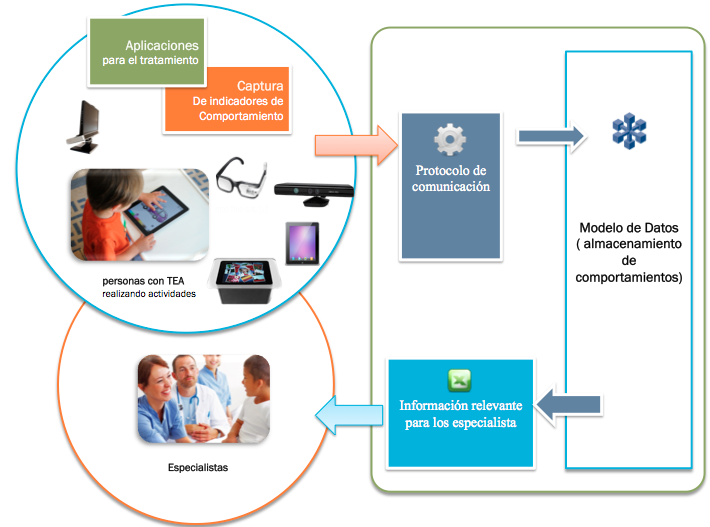
\includegraphics[width=15cm]{mono.png}
\end{center}
\caption{Dise\~no conceptual de la plataforma}
\end{figure}

En la figura 1 se describe el comportamiento de la plataforma que almacenara los 
indicadores capturados,  por un lado tenemos las aplicaciones que se utilizan para 
el tratamiento de los ni\~nos con TEA y un componente adicional que capturara los 
indicadores de comportamiento, una vez finalizada la captura de esta informaci\'on, 
ser\'a exportada a la plataforma a trav\'es de un protocolo de comunicaci\'on, quien 
realizara el nexo de la aplicaci\'on con el repositorio central, en donde ser\'an 
almacenados todos aquellos comportamientos capturados, en un an\'alisis 
posterior dichos datos almacenados podr\'an ser exportados a una planilla de
 calculo en donde podr\'an ser analizados. 

\section{Objetivos}
\label{obj}

\subsection{Objetivos generales}
Desarrollar una plataforma que permita el almacenamiento de indicadores de comportamiento 
generados por herramientas tecnol\'ogicas.


\subsection{Objetivos espec\'ificos}

\begin{itemize}
    \item Identificar los indicadores de comportamiento importantes para los especialistas, 
    a partir de la investigaci\'on del dominio del autismo con especialistas en el \'area.   
    
    \item Dise\~nar e implementar  un modelo de datos que permite almacenar los valores 
    de cada uno de los indicadores de comportamiento. en plataforma basada en cloud-computing
    
    \item Dise\~nar e implementar protocolo de comunicaci\'on basado en servicios web 
    entre aplicaciones y repositorio.
    
    \item Implementar un cliente que entregue indicadores a la plataforma principal, 
    dentro de una aplicaci\'on.
    
\end{itemize}




\section{Metodolog\'ia}
\label{metod}


Metodolog\'ia de desarrollo: Cascada Incremental \\
El m\'etodo que se utilizar\'a en este trabajo ser\'a la metodolog\'ia h\'ibrida, 
que contempla parte de desarrollo es cascada y otra de desarrollo incremental. 
En la actualidad se utilizan varias formas de gestionar los diferentes formas 
de desarrollar software, y a partir de las caracter\'isticas de la herramienta a 
fabricar, se adecua a una metodolog\'ia hibrida.



\begin{figure}[htb]
\begin{center}
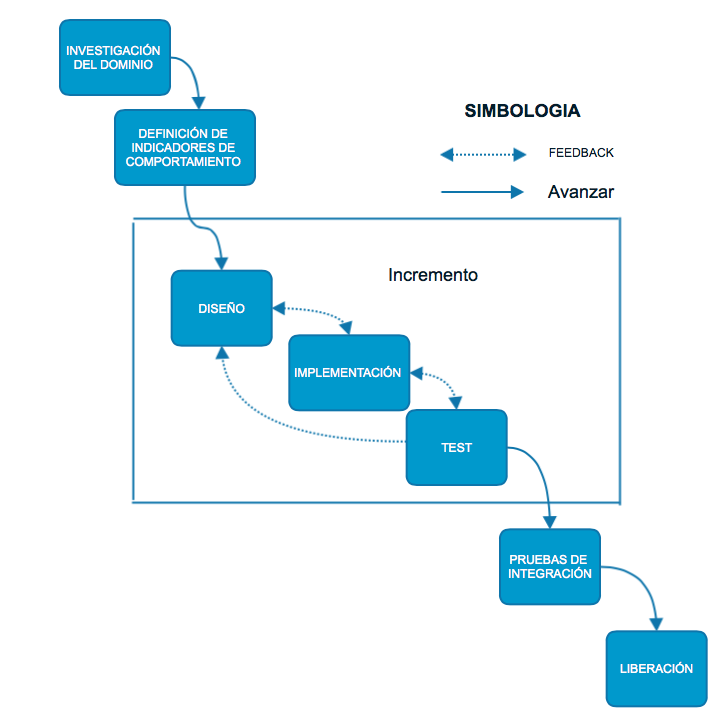
\includegraphics[width=8cm]{metodologia.png}
\end{center}
\caption{Metodolog\'ia de desarrollo del trabajo de t\'itulo}
\end{figure}



\newpage
\clearpage

\section{Planificaci\'on}
\label{plan}

Plan de desarrollo para lograr los objetivos planteados.

%% desarrollo tabla 1

\begin{table}[htf]
\begin{tabular}{| p{4cm} | c | c | p{3cm}  | p{2.5cm} |}
\hline

\multicolumn{5}{|c|}{\textbf{\textit{Planificaci\'on de Seminario de T\'itulo I 2014}}} \\ \hline \hline
\textit{\textbf{Actividades}} & 
\textit{\textbf{Inicio}} & 
\textit{\textbf{T\'ermino}} & 
\centering \textit{\textbf{Recurso}} & 
\textit{\textbf{Producto}} \\ \hline \hline
\textbf{Etapa 1: Propuesta de trabajo t\'itulo.} & 
\textbf{17/03/2014} & 
\textbf{04/04/2014} & 
\textbf{Profesor Gu\'ia, Documentos.} & 
\textbf{Propuesta Trabajo de T\'itulo} \\ \hline


Reunion 1 - Lineamiento trabajo de t\'itulo& 
18/03/2014 & 
18/03/2014 &  
Profesor gu\'ia & 
Propuesta de TT, Minuta 1.1 \\ \hline

Reunion 2 - Profesor gu\'ia & 
25/04/2014 & 
25/04/2014 &  
Profesor gu\'ia & 
Borrador 1, Minuta 1.2\\ \hline

Reunion 3 - Profesor gu\'ia & 
01/05/2014 & 
01/05/2014 &  
Profesor gu\'ia & 
Borrador 2, Minuta 1.3 \\ \hline


\hline
\end{tabular}
\caption{Planificaci\'on Etapa I}
\end{table}





%% desarrollo tabla 2

\begin{table}[htf]
\begin{tabular}{| p{4cm} | c | c | p{3cm}  | p{2.5cm} |}
\hline

\multicolumn{5}{|c|}{\textbf{\textit{Planificaci\'on de Seminario de T\'itulo I 2014}}} \\ \hline \hline
\textit{\textbf{Actividades}} & 
\textit{\textbf{Inicio}} & 
\textit{\textbf{T\'ermino}} & 
\centering \textit{\textbf{Recurso}} & 
\textit{\textbf{Producto}} \\ \hline \hline
\textbf{Etapa 2: Marco Conceptual, definici\'on del problema.} & 
\textbf{05/04/2014} & 
\textbf{25/04/2014} & 
\textbf{Profesor Gu\'ia, Libros, Internet, Expertos del dominio} & 
\textbf{Marco concept. def problema. An\'alisis de pautas e ind iniciales de comportamiento} \\ \hline


Reunion profesor gu\'ia & 
08/04/2014 & 
08/04/2014 &  
Expertos del dominio, Profesor gu\'ia & 
Borrador 1 - Minuta 2.1\\ \hline

Reunion profesor gu\'ia & 
15/04/2014 & 
15/04/2014 &  
Expertos del dominio, Profesor gu\'ia & 
Borrador 2 - Minuta 2.2 \\ \hline

Reunion profesor gu\'ia & 
22/04/2014 & 
22/04/2014 &  
Expertos del dominio, Profesor gu\'ia & 
Borrador 3 - Minuta 2.3\\ \hline


\hline
\end{tabular}
\caption{Planificaci\'on Etapa 2}
\end{table}



\newpage
\clearpage


%% desarrollo tabla 3

\begin{table}[htf]
\begin{tabular}{| p{4cm} | c | c | p{3cm}  | p{2.5cm} |}
\hline

\multicolumn{5}{|c|}{\textbf{\textit{Planificaci\'on de Seminario de T\'itulo I 2014}}} \\ \hline \hline
\textit{\textbf{Actividades}} & 
\textit{\textbf{Inicio}} & 
\textit{\textbf{T\'ermino}} & 
\centering \textit{\textbf{Recurso}} & 
\textit{\textbf{Producto}} \\ \hline \hline
\textbf{Etapa 3: Dise\~no de la soluci\'on.} & 
\textbf{26/04/2014} & 
\textbf{16/05/2014} & 
\textbf{Alumno, Profesor gu\'ia} & 
\textbf{Primera iteraci\'on de desarrollo (an\'alisis, dise\~no, implementaci\'on, modelo de datos y documentaci\'on} \\ \hline


Reunion profesor gu\'ia & 
29/04/2014 & 
29/04/2014 &  
Alumno, Profesor gu\'ia & 
An\'alisis, dise\~no ( borrador 1, Minuta 3.1)\\ \hline

Reunion profesor gu\'ia & 
06/05/2014 & 
06/05/2014 &  
Alumno, Profesor gu\'ia & 
Implementaci\'on (Borrador 2, Minuta 3.2) \\ \hline

Reunion profesor gu\'ia & 
13/05/2014 & 
13/05/2014 &  
Alumno, Profesor gu\'ia & 
Documentaci\'on (Minuta 3.3\\ \hline


\hline
\end{tabular}
\caption{Planificaci\'on Etapa 3}
\end{table}



\newpage
\clearpage

%% desarrollo tabla 4

\begin{table}[htf]
\begin{tabular}{| p{4cm} | c | c | p{3cm}  | p{2.5cm} |}
\hline

\multicolumn{5}{|c|}{\textbf{\textit{Planificaci\'on de Seminario de T\'itulo I 2014}}} \\ \hline \hline
\textit{\textbf{Actividades}} & 
\textit{\textbf{Inicio}} & 
\textit{\textbf{T\'ermino}} & 
\centering \textit{\textbf{Recurso}} & 
\textit{\textbf{Producto}} \\ \hline \hline
\textbf{Etapa 4: Implementaci\'on.} & 
\textbf{26/04/2014} & 
\textbf{16/05/2014} & 
\textbf{Alumno, Profesor gu\'ia} & 
\textbf{2da  iteraci\'on de desarrollo (an\'alisis, dise\~no implementaci\'on,) + documentaci\'on} \\ \hline


Reunion profesor gu\'ia & 
20/05/2014 & 
20/05/2014 &  
Alumno, Profesor gu\'ia & 
An\'alisis, Dise\~no, Implementaci\'on, Documentaci\'on, Minuta\\ \hline

Reunion profesor gu\'ia & 
27/05/2014 & 
27/05/2014 &  
Alumno, Profesor gu\'ia & 
An\'alisis, Dise\~no, Implementaci\'on, Documentaci\'on, Minuta\\ \hline

Reunion profesor gu\'ia & 
03/06/2014 & 
03/06/2014 &  
Alumno, Profesor gu\'ia & 
An\'alisis, Dise\~no, Implementaci\'on, Documentaci\'on, Minuta\\ \hline

Reunion profesor gu\'ia & 
10/06/2014 & 
10/06/2014 &  
Alumno, Profesor gu\'ia & 
An\'alisis, Dise\~no, Implementaci\'on, Documentaci\'on, Minuta\\ \hline

\hline
\end{tabular}

\end{table}



\newpage
\clearpage



\begin{table}[htf]
\begin{tabular}{| p{4cm} | c | c | p{3cm}  | p{2.5cm} |}
\hline

\multicolumn{5}{|c|}{\textbf{\textit{Planificaci\'on de Seminario de T\'itulo I 2014}}} \\ \hline \hline
\textit{\textbf{Actividades}} & 
\textit{\textbf{Inicio}} & 
\textit{\textbf{T\'ermino}} & 
\centering \textit{\textbf{Recurso}} & 
\textit{\textbf{Producto}} \\ \hline \hline

Reunion profesor gu\'ia & 
17/06/2014 & 
17/06/2014 &  
Alumno, Profesor gu\'ia & 
An\'alisis, Dise\~no, Implementaci\'on, Documentaci\'on, Minuta\\ \hline

Reunion profesor gu\'ia & 
24/06/2014 & 
24/06/2014 &  
Alumno, Profesor gu\'ia & 
An\'alisis, Dise\~no, Implementaci\'on, Documentaci\'on, Minuta\\ \hline

Reunion profesor gu\'ia & 
01/07/2014 & 
01/07/2014 &  
Alumno, Profesor gu\'ia & 
An\'alisis, Dise\~no, Implementaci\'on, Documentaci\'on, Minuta\\ \hline

\hline
\end{tabular}
\caption{Planificaci\'on Etapa 4}
\end{table}




\newpage
\clearpage

\section{Recursos}
\label{rec}


\subsection{Recursos Humanos}
  \begin{itemize}
    \item Profesor Gu\'ia
    \item Experto del dominio (Trastornos del Espectro Autista)
  \end{itemize}
\subsection{Hardware}
\begin{itemize}
    \item Computador: Procesador 2,3 GHz Intel Core i5, Memoria 8 GB 1333 MHz DDR3, 
    500GB de disco duro
  \end{itemize}
\subsection{Software}
  \begin{itemize}
    \item Plataforma de alta escalabilidad (hadoop).
    \item Motor de base de datos (Nosql)
    \item Netbeans (servicio rest, webservice)
  \end{itemize}

\subsection{Otros}
  \begin{itemize}
    \item Internet 
    \item Libros  
    \item Publicaciones de revistas cient\'ificas del dominio 
    (bibliotecas digitales extranjeras)  
  \end{itemize}

\newpage
\clearpage

\bibliography{propuesta}
\bibliographystyle{plain}
\end{document} 